\documentclass[aspectratio=169]{beamer}
\usetheme{SimplePlus}

\usepackage{tikz}
\usepackage{pgfplots}
\usepackage{amsmath}
\usepackage{amssymb}
\usepackage{bm}
\usepackage{mathtools}
\usepackage{algpseudocode}
\DeclareMathOperator{\grad}{\nabla}
\renewcommand{\P}{\mathbb{P}}
\newcommand{\R}{\mathbb{R}}

\title[Finite Elements I]{Finite Elements Theory}
\author{Nicol\'as A. Barnafi}
\date{\today}


\begin{document}

\begin{frame}
    \titlepage
\end{frame}

\section{Motivation}

\begin{frame}{Motivation: Céa's Lemma and Interpolation}
    Let $V$ be Hilbert, $a(\cdot,\cdot)$ a elliptic/continuous bilinear form, and $V_h \subset V$ discrete space. We obtained previously:

    $$ \|u - u_h\|_V \leq \frac{M}{\alpha} \inf_{v_h \in V_h} \|u - v_h\|_V$$

    \vspace{0.3cm}
    \pause Assume we have an \textbf{interpolation} $\Pi_h : V \to V_h$ with 

        $$ \| u - \Pi_h u \| \leq C h^\ell, \quad\text{then}$$ \pause

        $$ \|u - u_h\|_V \leq \frac{M}{\alpha} \inf_{v_h \in V_h} \|u - v_h\|_V \alert{\leq \frac{M}{\alpha} \|u - \Pi_h u\|_V \leq \frac{MC}{\alpha} h^\ell }$$

        This is usually \emph{optimal}.
\end{frame}

\section{Geometric Setup}

\begin{frame}{Geometric Setup: Domain and Mesh Size}
    Consider a 1D domain $\Omega = (a, b)$. We define a partition (mesh) $\mathcal{T}_h$:

    $$ a = x_0 < x_1 < \dots < x_{N-1} < x_N = b $$

    \begin{itemize}
        \item \textbf{Elements:} $I_j = (x_{j-1}, x_j)$ for $j = 1, \dots, N$.
        \item \textbf{Nodes:} The set of points $\{x_j\}_{j=0}^N$.
        \item \textbf{Local Element Size:} $h_j = x_j - x_{j-1}$.
        \item \textbf{Global Mesh Size:} The fundamental parameter for asymptotic analysis:
        $$ h = \max_{1 \leq j \leq N} h_j $$
    \end{itemize}
\end{frame}

\section{Linear FE Properties}

\begin{frame}{Linear Finite Elements: Space and Basis}
    We define the space of continuous, piecewise linear functions:
    $$ V_h = \{ v_h \in C^0(\bar{\Omega}) : v_h|_{I_j} \in \mathcal{P}^1(I_j) \quad \forall j=1,\dots,N \} $$

    \textbf{Proposition:} $V_h = \text{span}_{i=0}^N\{\varphi_i\}$, with $\varphi_i$ hat functions.

    \textbf{Proof:}\pause
    \begin{itemize}[<+->]
        \item By construction, if $v_h\in V_h$: 
            $$ v_h = \sum_i v_h(x_i) \varphi_i. $$
        \item Set $v_h = \sum_i v^i \varphi_i = 0$, then
                $$ v_h(x_j) = v^i \varphi_i(x_j) = v^i \delta_{ij} = v^j = 0, $$
                and thus they are linearly independent.
    \end{itemize}
    \qed
\end{frame}

\begin{frame}{$H^1$ Conformity}
    \textbf{Proposition:} The space $V_h$ is conforming in $H^1(\Omega)$, i.e., $V_h \subset H^1(\Omega)$.

    \textbf{Proof:}
    Let $v_h \in V_h$. We must show that $v_h \in L^2(\Omega)$ and possesses a weak derivative $v_h' \in L^2(\Omega)$.
    \begin{itemize}
        \item They belong to $L^2$ because $v_h\in C^0\subset L^2$.
        \item We now compute gradient: 
        \begin{align*}
            \langle v_h', \varphi\rangle &= \sum_{j=1}^N \int_{I_j} v_h \varphi' dx = \sum_{j=1}^N \left( \underbrace{[v_h \varphi]_{x_{j-1}}^{x_j}}_\text{telescopic} - \int_{I_j} \underbrace{\partial_x v_h}_{d^j \coloneqq} \varphi dx \right) \tag{Integration by parts on $I_j$} \\
            &= \int_\Omega \sum_j I_j d^j \varphi dx
        \end{align*}
        Thus, $v_h' = \sum_j I_j d^j\in L^\infty(\Omega)\subset L^2(\Omega)$. \qed
    \end{itemize}
\end{frame}


\begin{frame}{Degrees of Freedom via the Dual Space}
    Consider $V_h^*$ the dual of $V_h$. We define the \textbf{global degrees of freedom (DOFs)} as linear functionals $\Sigma_h = \{\sigma_0, \dots, \sigma_N\} \subset V_h^*$ defined by:
    $$ \sigma_i(v_h) = v_h(x_i) \quad \forall i=0,\dots,N $$

    \textbf{Proposition (Unisolvence):} $\Sigma_h$ forms a basis for $V_h^*$ that is dual to $\{\varphi_i\}$.

    \textbf{Proof:} \pause
    \begin{itemize}[<+->]
        \item They are linearly independent: 
            $$ 0 = \sum_i c^i\sigma_i(\varphi_j) = \sum_i c^i \delta_{ij} = c^j $$
        \item They span space: Consider $v_h$ in $V_h$ and we look for coefficients $c^i$ such that
            $$ \sigma_h(v_h) = \sum_i c^i \sigma_i(v_h) = \sum_{i,j} c^i v^j \delta_{ij} = \sum_{i} c^i v^i $$
            and setting $v^\ell = 1$ only for $\ell=i$ yields $c^i = \sigma_h(\varphi_i)$.  \qed
    \end{itemize}
\end{frame}


\begin{frame}{The Interpolator Operator}
    \textbf{Definition:} The global interpolation operator $\Pi_h : C^0(\bar{\Omega}) \to V_h$ is defined by:
    $$ \Pi_h u(x) = \sum_{i=0}^N \sigma_i (u) \phi_i(x) = \sum_{i=0}^N u(x_i) \phi_i(x) $$

    Equivalently, using the DoFs:
    $$ \sigma_i(\Pi_h u) = \sigma_i(u) \quad \forall i=0,\dots,N $$

    Note: $\Pi_h$ is a projection, meaning $\Pi_h(\Pi_h u) = \Pi_h u$.

    We now study the local interpolation error $e = u - \Pi_h u$ on a single element $I_j$.
\end{frame}
\begin{frame}[t]{Continuity of the Interpolator in $H^1(\Omega)$}
    \textbf{Theorem:} $\exists C > 0$ such that $\|\Pi_h u\|_{H^1(\Omega)} \leq C \|u\|_{H^1(\Omega)}$.
    
    \textbf{Proof:} 
        \begin{itemize}
            \item<1-> $\| \Pi_h u \|_{L^2(\Omega)} \leq C \| u\|_1$
                   \only<1>{ 
                       \begin{enumerate}
                            \item In 1D  $\|u\|_{L^2(\Omega)} \leq |\Omega|\|u\|_{L^\infty(\Omega)} \leq |\Omega| C_{emb} \|u\|_{H^1(\Omega)}$ (Sobolev Embedding).

                            \item $$ \|\Pi_h u\|_{L^2(\Omega)}^2 \leq |\Omega| \|\Pi_h u\|_{L^\infty(\Omega)}^2 \leq |\Omega| \|u\|_{L^\infty(\Omega)}^2 \leq |\Omega| C_{emb} \|u\|_{H^1(\Omega)}^2 $$
                        \end{enumerate}
                    }
                \item<2-> $ \| (\Pi_h u)' \|_{I_j} \leq C \|u \|_{H^1(I_j)} $ 
                    \only<2>{
                        \begin{enumerate}
                            \item On $I_j$, $(\Pi_h u)' = \frac{u(x_j) - u(x_{j-1})}{h_j}$.
                            \item We bound extremal differences:
                                \begin{align*}
                                    |u(x_j) - u(x_{j-1})|^2 &= \left| \int_{I_j} u'(x) dx \right|^2 \tag{Fund. Thm. of Calculus} \\
                                    &\leq \left( \int_{I_j} 1^2 dx \right) \left( \int_{I_j} |u'(x)|^2 dx \right) = h_j \|u'\|^2_{L^2(I_j)} \tag{Cauchy-Schwarz}
                                \end{align*}
                            \item We bound the $H^1$ semi-norm:
                                $$ |\Pi_h u|_{H^1(I_j)}^2 = \int_{I_j} \left| \frac{u(x_j) - u(x_{j-1})}{h_j} \right|^2 dx = \frac{|u(x_j) - u(x_{j-1})|^2}{h_j} \leq \|u'\|^2_{L^2(I_j)}  $$
                        \end{enumerate}
                    }
    
                \item<3-> Sum over all $I_j$. \qed
        \end{itemize}
\end{frame}
\begin{frame}{Interpolation: $H_0^1$ convergence rate}
    \textbf{Theorem:} Let $u \in H^2(I_j)$. Then $|u - \Pi_h u|_{H^1(I_j)} \leq h_j \|u''\|_{L^2(I_j)}$. \pause

    \textbf{Proof:} Let $e = u - \Pi_h u$. Since $e(x_{j-1}) = e(x_j) = 0$, by Rolle's Theorem, $\exists \xi \in I_j$ such that $e'(\xi) = 0$. For any $x \in I_j$:
    \begin{align*}
        e'(x) &= \int_\xi^x e''(t) dt \tag{Fund. Thm. of Calculus} \\
        |e'(x)| &\leq \left( \int_\xi^x 1^2 dt \right)^{1/2} \left( \int_\xi^x |e''(t)|^2 dt \right)^{1/2} \tag{Cauchy-Schwarz} \\
        |e'(x)|^2 &\leq h_j \int_{I_j} |e''(t)|^2 dt = h_j \|e''\|_{L^2(I_j)}^2 \tag{Bounding integral domain} \\
        \int_{I_j} |e'(x)|^2 dx &\leq \int_{I_j} h_j \|e''\|_{L^2(I_j)}^2 dx = h_j^2 \|e''\|_{L^2(I_j)}^2 \tag{Integrate over $I_j$}
    \end{align*}
    Taking the square root, and noting $e'' = u'' - (\Pi_h u)'' = u''$ (since $\Pi_h u \in \mathcal{P}^1$), we get $|e|_{H^1(I_j)} \leq h_j \|u''\|_{L^2(I_j)}$. \qed
\end{frame}

\begin{frame}{Interpolation Error: $L^2$ Norm Rate}
    \textbf{Theorem:} Let $u \in H^2(I_j)$. Then $\|u - \Pi_h u\|_{L^2(I_j)} \leq h_j^2 \|u''\|_{L^2(I_j)}$.

    \textbf{Proof:} Let $e = u - \Pi_h u$. Since $e(x_{j-1}) = 0$, for any $x \in I_j$:
    \begin{align*}
        e(x) &= \int_{x_{j-1}}^x e'(t) dt \tag{Fund. Thm. of Calculus} \\
        |e(x)| &\leq \left( \int_{x_{j-1}}^x 1^2 dt \right)^{1/2} \left( \int_{x_{j-1}}^x |e'(t)|^2 dt \right)^{1/2} \tag{Cauchy-Schwarz} \\
        |e(x)|^2 &\leq h_j \|e'\|_{L^2(I_j)}^2 \tag{Bounding integral domain} \\
        \int_{I_j} |e(x)|^2 dx &\leq \int_{I_j} h_j \|e'\|_{L^2(I_j)}^2 dx = h_j^2 \|e'\|_{L^2(I_j)}^2 \tag{Integrate over $I_j$}
    \end{align*}
    From the previous theorem, $\|e'\|_{L^2(I_j)}^2 \leq h_j^2 \|u''\|_{L^2(I_j)}^2$. Substitution yields:
    $$ \|e\|_{L^2(I_j)}^2 \leq h_j^4 \|u''\|_{L^2(I_j)}^2 \implies \|e\|_{L^2(I_j)} \leq h_j^2 \|u''\|_{L^2(I_j)} $$ \qed
\end{frame}

\section{The Finite Element Formalism}

\begin{frame}{The Finite Element Definition (Ciarlet)}
    \textbf{Definition:} A Finite Element is a triple $(K, \mathcal{P}, \Sigma)$ where:
    \begin{enumerate}
        \item $K \subset \mathbb{R}^d$ is a closed, bounded subset with non-empty interior (geometric element).
        \item $\mathcal{P}$ is a finite-dimensional vector space of functions on $K$ (shape functions).
        \item $\Sigma$ is a set of unisolvent linear functionals on $\mathcal{P}$ (the degrees of freedom).
    \end{enumerate}

    \pause \textbf{Proposition:} The 1D linear element is a finite element.

    \textbf{Proof:} Let $\hat{K} = [-1, 1]$. We define the reference triple $(\hat{K}, \hat{\mathcal{P}}, \hat{\Sigma})$:
    \begin{align*}
        \hat{\mathcal{P}} &= \mathcal{P}^1(\hat{K}) = \text{span}\{1-\hat{x}, \hat{x}\} \\
        \hat{\Sigma} &= \{ \hat{\sigma}_1(\hat{v}) = \hat{v}(-1), \hat{\sigma}_2(\hat{v}) = \hat{v}(1) \} \tag{Clearly unisolvent}
    \end{align*}
    Any arbitrary element $I_j = [x_{j-1}, x_j]$ is generated via the affine map $F_j : \hat{K} \to I_j$, $x = F_j(\hat{x}) = \frac{x_{j-1}+x_j}{2} + \hat{x}\frac{h_j}{2}$. \qed
\end{frame}

\begin{frame}[fragile]{Higher-Order Lagrange Elements}
    We can construct higher-order elements by choosing $\mathcal{P} = \mathcal{P}^k(K)$ for $k \geq 2$. The DOFs $\Sigma$ evaluate the function at $k+1$ equidistant nodes in $K$.

    \begin{center}
    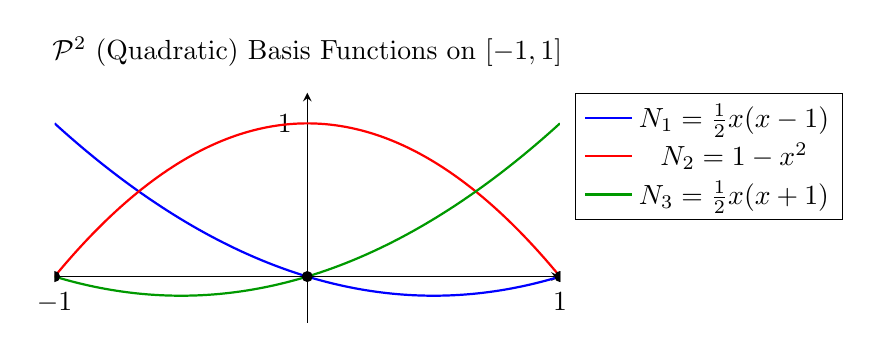
\begin{tikzpicture}
        \begin{axis}[
            width=8cm, height=4.5cm,
            domain=-1:1, samples=100,
            axis lines=middle,
            ymin=-0.3, ymax=1.2,
            xtick={-1, 0, 1},
            xticklabels={$-1$, $0$, $1$},
            ytick={1},
            title={$\mathcal{P}^2$ (Quadratic) Basis Functions on $[-1,1]$},
            legend pos=outer north east
        ]
        \addplot[thick, blue] {0.5*x*(x-1)}; \addlegendentry{$N_1 = \frac{1}{2}x(x-1)$}
        \addplot[thick, red] {1-x^2}; \addlegendentry{$N_2 = 1-x^2$}
        \addplot[thick, green!60!black] {0.5*x*(x+1)}; \addlegendentry{$N_3 = \frac{1}{2}x(x+1)$}

        \fill[black] (axis cs:-1,0) circle (2pt);
        \fill[black] (axis cs:0,0) circle (2pt);
        \fill[black] (axis cs:1,0) circle (2pt);
        \end{axis}
    \end{tikzpicture}
    \end{center}
\end{frame}

\begin{frame}{Convergence Rates for Higher-Order Elements}
    By extending the Taylor expansion and scaling arguments to polynomial spaces of degree $k$, one obtains the generalized interpolation estimates.

    For $u \in H^{k+1}(\Omega)$ and a mesh with size $h$:

    \vspace{0.3cm}
    \textbf{1. $L^2$ Error Estimate:}
    $$ \|u - \Pi_h u\|_{L^2(\Omega)} \leq C h^{k+1} |u|_{H^{k+1}(\Omega)} $$

    \textbf{2. $H^1$ Semi-norm Error Estimate:}
    $$ |u - \Pi_h u|_{H^1(\Omega)} \leq C h^k |u|_{H^{k+1}(\Omega)} $$

    \vspace{0.3cm}
    Applying Céa's Lemma (5.2), the Galerkin approximation inherits these optimal rates in the energy norm:
    $$ \|u - u_h\|_{H^1(\Omega)} \leq C h^k |u|_{H^{k+1}(\Omega)} $$
\end{frame}

\begin{frame}
    \titlepage
\end{frame}

\end{document}

